\documentclass[a4paper,12pt]{report}

%Packages Used
\usepackage{amssymb,latexsym,amsmath}     % Standard packages
\usepackage{setspace}
\usepackage{sectsty}
\usepackage{titlesec}
\usepackage{hyperref}
\usepackage{bookmark}
\usepackage{graphics,graphicx}
\usepackage{tikz}
\usepackage{mathtools}
\usepackage{graphicx}
\usepackage{amssymb}
\usepackage{esvect}
\usepackage{chngcntr}
\usepackage{indentfirst}

\DeclarePairedDelimiter\abs{\lvert}{\rvert}%
\DeclarePairedDelimiter\norm{\lVert}{\rVert}%


\bookmarksetup{
  numbered,
  open
}
\renewcommand*{\thesection}{\arabic{section}}
\onehalfspacing

\newcommand{\suchthat}{\;\ifnum\currentgrouptype=16 \middle\fi|\;}

%Margins
\addtolength{\textwidth}{1.0in}
\addtolength{\textheight}{1.00in}
\addtolength{\evensidemargin}{-0.75in}
\addtolength{\oddsidemargin}{-0.75in}
\addtolength{\topmargin}{-.50in}

%%%%%%%%%%%%%%%%%%%%%%%%%%%%%% 
% Theorem/Proof Environments %
%%%%%%%%%%%%%%%%%%%%%%%%%%%%%%
\newtheorem{theorem}{Theorem}
\newenvironment{proof}{\noindent{\bf Proof:}}{$\hfill \Box$ \vspace{10pt}}
\sectionfont{\fontsize{12}{15}\selectfont}
\subsectionfont{\fontsize{12}{15}\selectfont}
\titlespacing*{\section}{0.5pt}{0.25\baselineskip}{0.25\baselineskip}




\begin{document}
\noindent
Yufei Lin

\noindent
Final Essay

\noindent
Apr \(30^{th}\) 2020

\begin{center}
\textbf{Final Essay}
\end{center}

\section*{Abstract}

This research seeks to improve the existing cellular automata models for simulating sustainable city development. The existing literature has taken land use dynamics as a direct representation of city development. This literature has accounted for the economic, environmental, and social factors affecting land use transition probabilities within a context of a growing city. We will expand upon this model to investigate how changes to the transition probabilities could influence the way a city develops. 

\section{Introduction}

In this research, we started building out a simple land simulation system with four different land use types: Nature, Residential, Commercial and Industrial, where all cells change follows a specific transition matrix. Then, we expand this model to look at how neighbouring cells would effect the transition probabilities of an existing cell by first looking at a simpler model where we only take in the different number of land types into account, and then look at a combination of different number of land use types and a set of given transition matrices. And, we look at the percentage of nature and residential, and the average distance from a cell to all three other types of land uses.  

\section{Cellular Automata Simulation of City Development}

In this simplified model, we have only four land use types, Nature, Residential, Commercial, and Industrial. In this process, we have defined a $10\times 10$ board to describe a city. Then, we are defining a few different transition matrices to look at the development of the city. This transition matrix is looking at the transition probabilities of the city development within 10 years. 

\subsection{Preset Transition Matrix}

The transition matrix is defined to look at the probabilities for the cell to change to another land use types. This matrix is obtained from \textcolor{red}{a previous article}. And the matrix is as the following:
\begin{table}[ht]
\centering
\begin{tabular}{l|l|l|l|l}
            & Nature & Residential & Commercial & Industrial \\ \hline
Nature      & 0.6    & 0.1         & 0.15       & 0.15       \\ \hline
Residential & 0.05   & 0.8         & 0.1        & 0.05       \\ \hline
Commercial  & 0.05   & 0.15        & 0.7        & 0.1        \\ \hline
Industrial  & 0.08   & 0.02        & 0.1        & 0.8       
\end{tabular}
\\[10pt]
\caption{Preset Transition Matrix}
\end{table}

\pagebreak

Since the land is defined as a matrix with numbers, we reshape the land into a $100\times 4$ matrix that marks the land use type for each cell, and multiply this with the $4\times 4$ transition matrix to obtain the probabilities for each cell to change. Then we use a stochastic probability to represent the next generation of the cell.  

\subsection{A Set of Transition Rules}

This section, we look at a collection of rules to describe the neighbourhood behaviour of a cell based on the transition matrix. At this particular part, we first define four transition matrices, where we look at if the surroundings of the cell is purely one of the four types. And the matrices are defined as the following. 

\begin{table}[ht]
\centering
\begin{tabular}{l|l|l|l|l}
            & Nature & Residential & Commercial & Industrial \\ \hline
Nature      & 0.6    & 0.1         & 0.15       & 0.15       \\ \hline
Residential & 0.05   & 0.8         & 0.1        & 0.05       \\ \hline
Commercial  & 0.05   & 0.15        & 0.7        & 0.1        \\ \hline
Industrial  & 0.08   & 0.02        & 0.1        & 0.8       
\end{tabular}
\\[10pt]
\caption{All Nature Rules}
\end{table}

\begin{table}[ht]
\centering
\begin{tabular}{l|l|l|l|l}
            & Nature & Residential & Commercial & Industrial \\ \hline
Nature      & 0.84   & 0.05        & 0.06       & 0.05       \\ \hline
Residential & 0.03   & 0.52        & 0.39       & 0.06       \\ \hline
Commercial  & 0.01   & 0.20        & 0.61       & 0.18       \\ \hline
Industrial  & 0.2    & 0.02        & 0.18       & 0.6       
\end{tabular}
\\[10pt]
\caption{All Residential Rules}
\end{table}

\begin{table}[ht]
\centering
\begin{tabular}{l|l|l|l|l}
            & Nature & Residential & Commercial & Industrial \\ \hline
Nature      & 0.5    & 0.12        & 0.3        & 0.08       \\ \hline
Residential & 0.02   & 0.8         & 0.1        & 0.08       \\ \hline
Commercial  & 0.04   & 0.18        & 0.6        & 0.18       \\ \hline
Industrial  & 0.19   & 0.04        & 0.26       & 0.51      
\end{tabular}
\\[10pt]
\caption{All Commercial Rules}
\end{table}

\begin{table}[ht]
\centering
\begin{tabular}{l|l|l|l|l}
            & Nature & Residential & Commercial & Industrial \\ \hline
Nature      & 0.45   & 0.01        & 0.18       & 0.36       \\ \hline
Residential & 0.2    & 0.5         & 0.1        & 0.2        \\ \hline
Commercial  & 0.25   & 0.02        & 0.45       & 0.28       \\ \hline
Industrial  & 0.04   & 0           & 0.16       & 0.8       
\end{tabular}
\\[10pt]
\caption{All Industrial Rules}
\end{table}

\pagebreak
Then we obtain the cell's land use type, and get the transition vector for that particular type from the above four matrices. Then we multiply the vector with the percentage of each land use type and add them up together to get the new transition vector. After that we use a stochastic probability to get the next generation for the cell.  

\subsection{Result Comparison}

We started from looking at the city of a $10\times 10$ grid with the city center locates at $(6,3), (6,4), (7,3), (7,4)$. Therefore, the city starts from the following graph:

\begin{figure}[h]
\centering
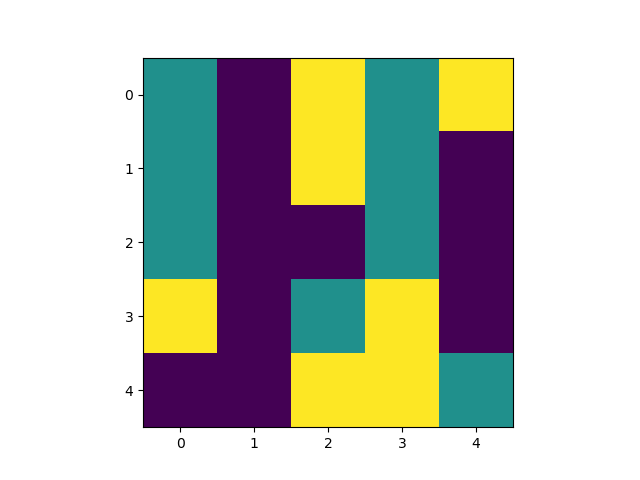
\includegraphics[scale=0.6]{../output/Original.png}
\caption{Original Land}
\end{figure}

\pagebreak
From using the given transition matrix cellular automata, we have the following result:

\begin{figure}[h]
\centering
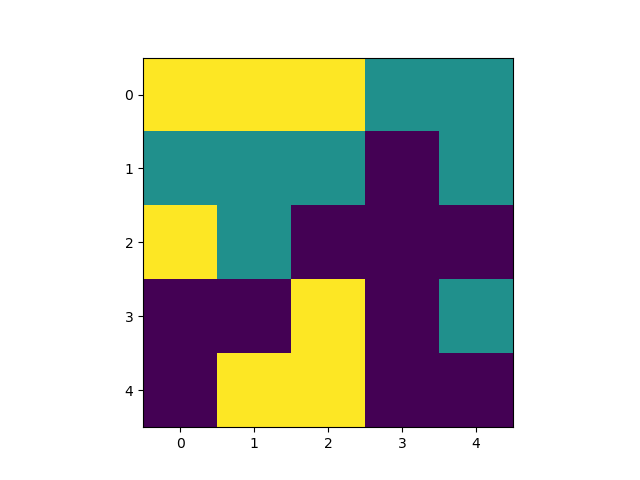
\includegraphics[scale=0.6]{../output/Gen-10.png}
\caption{100 Years Later}
\end{figure}

From using the cellular automata with a set of transition rules, we have the following result:

\begin{figure}[h]
\centering
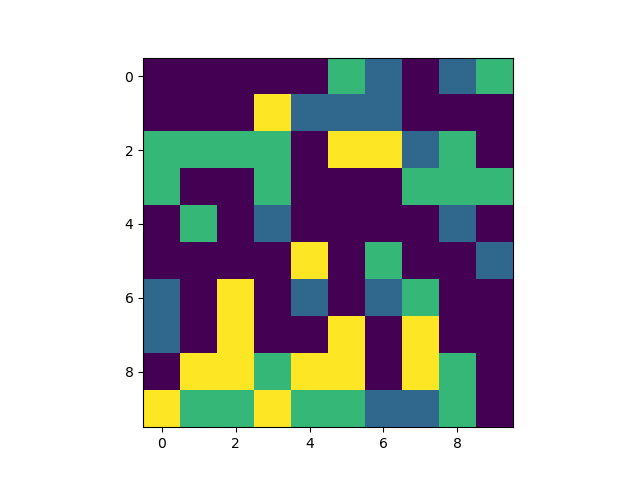
\includegraphics[scale=0.6]{../output/Land3/Land3-Gen-10.png}
\caption{100 Years Later}
\end{figure}
\end{document}